\section{Introduction}

Tomographic reconstruction is a problem of inverting Radon transformation in 2D or 3D in order to recover unknown attenuation $\mu(.)$ from the set of line integrals that represents measured data. Analytical methods are based on a direct expression for the inverse or an approximation of it, see \cite{Feldkamp1984, Tuy1983, Katsevich2004}. Analytical formulas do not include discretization, which must be considered separately.

Algebraic methods, on the other hand, rely on the formulation of a projection operator that models X-ray absorption and accounts for discretization. The CT operator $\mathbf{A} \in \mathbb{R}^{m \times n}$ directly describes the relationship between the voxel attenuation values in the imaged sample $\vec{x} \in \mathbb{R}^n$ and the pixel values on the detector $\vec{b} \in \mathbb{R}^m$ so that
\begin{equation}
    \mathbf{A} \vec{x} = \vec{b}.
    \label{eq:fundament}
\end{equation}
Algebraic methods aim to compute the vector $\vec{x}_{min}$ that minimizes certain functional, such as the squared residual error for given projection data $\boldsymbol{b}$, using an iterative process, see \cite{Rit2014,Kulvait2021}. The possibility to choose the proper search space for the solution, together with the variability of the form of the functional to minimize makes these methods a versatile tool for CT reconstruction. They are suitable for applications such as limited-angle reconstruction, a priori knowledge problems or time-dependent reconstruction of contrast agent dynamics in perfusion imaging, see for example \cite{Kulvait2022,Haseljic2021}.
%in various circumstances such as limited angle reconstruction, problems with apriori knowledge or the reconstruction of the time dependent contrast agent dynamics in scope of perfusion imaging, see for example \cite{Haseljic2021}.%, see for example \cite{}.

\begin{figure}
    \centering
    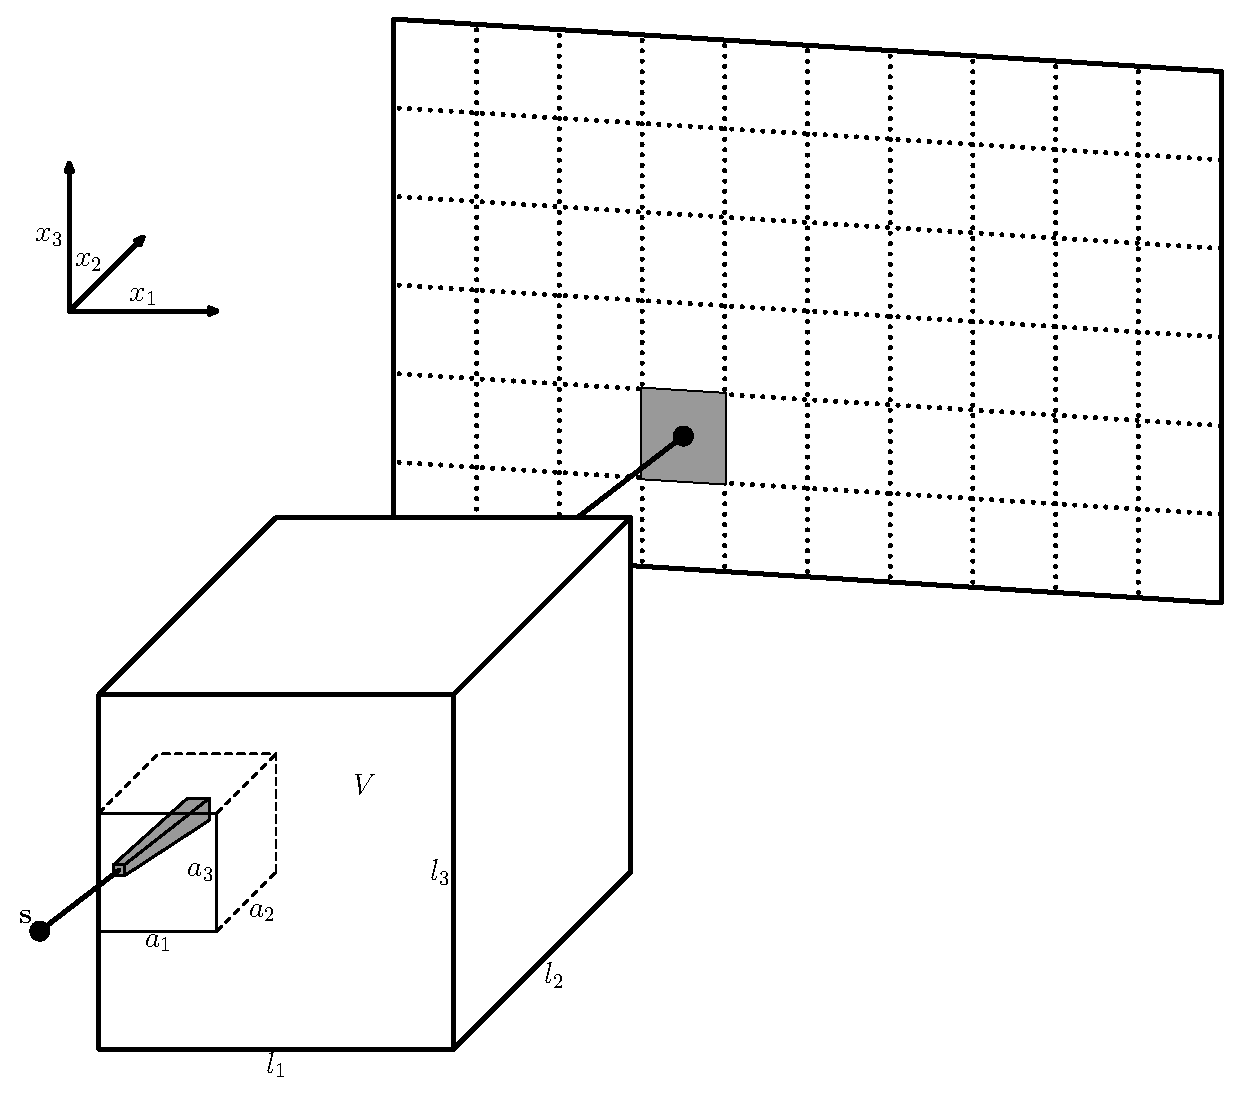
\includegraphics[width=0.45\textwidth]{projectionScheme-1.eps}
    \caption{The cutting voxel projector estimates the voxel contribution to the detected value at a particular pixel based on the volume of intersection of the voxel with all possible rays to that pixel.}
    \label{fig:problem_setup}
\end{figure}

Iterative methods require efficient and accurate evaluation of the actions of projection and backprojection operators. The projection operator acts on volume data $\vec{x}_{\mathrm{IN}} \in \mathbb{R}^n$  and returns the projection vector $\vec{b}_{\mathrm{OUT}} \in \mathbb{R}^m$ such that $\vec{b}_{\mathrm{OUT}} = \mathbf{A} \vec{x}_{\mathrm{IN}}$. The backprojection operator acts on projection vector $\vec{b}_{\mathrm{IN}} \in \mathbb{R}^n$ and returns the volume data $\vec{x}_{\mathrm{OUT}} \in \mathbb{R}^n$ such that $\vec{x}_{\mathrm{OUT}} = \mathbf{A}^\top \vec{b}_{\mathrm{IN}}$. Because the I/O latencies of data storage devices are high, it is prohibitive for typical CT systems to store the matrix $\mathbf{A}$ on disk and perform these matrix multiplications directly. Computing the projection and backprojection operators on the fly on current GPUs is typically orders of magnitude faster than working with the $\mathbf{A}$ matrix stored on disk. Therefore, there is a demand for fast and accurate projection and backprojection operators.

Ray casting/tracing projectors are well established not only in the context of CT imaging, but also in the context of computer graphics, see \cite{Siddon1985,Sramek2000,Zhao2003}. They track the ray cast from the source to the detector and add the values along the way to form the product of the geometry factors in $\mathbf{A}$ row with given vector of attenuation $\vec{x}_{\mathrm{IN}}$. Outer loop of these projectors is over the detector pixels, so they are scanning the matrix $\mathbf{A}$ row by row. Their accuracy is strongly dependent on the number of rays cast. Backprojection is typically slower than projection and, in addition, it is unable to capture the underlying physical process well, resulting in a strong geometric artefacts in reconstructions.

Footprint projectors on the other hand try to estimate for each voxel and position on the detector the length of the intersection of the voxel with the ray to that position. Their outermost loop is over voxels, so that they scan the matrix $\mathbf{A}$ column by column. Current implementations rely on the assumption that footprints can be approximated in each detector direction by very simple functions, for example by constants with a small support, see \cite{Man2004}, or by constants in the middle with linearly decaying tails on each side, so-called trapezoidal functions. Separable footprint projectors approximate blur on the detector due to a given voxel by product of two such functions, each for one detector dimension, see \cite{Long2010}. They extend the work of \cite{Man2004} and are considered state of the art CT projectors. The inaccuracies of this class of projectors are due to the fact that the actual footprints are generally not separable and thus do not satisfy assumptions about the shape of the footprint functions.
% The algorithm \cite{Long2010} also assumes certain geometric setting of the acquisition system. 

In this paper, we construct a projector that directly describes the voxel pixel correspondence by computing integrals over the volumes of voxel cuts projected onto a given pixel instead of averaging line integrals over rays passing through the voxels, see \figref{fig:problem_setup}. In order to accurately compute the projection of a given voxel onto a given pixel, we need to reformulate the problem using integral calculus to find the correspondence between the integrals over all rays passing through the voxel and the integrals over the voxel cut volume. This approach eliminates the need to cast a high number of rays towards a given pixel to increase accuracy, and also overcomes assumptions about the shapes of the footprints.
